\documentclass[a4paper,10pt,twoside]{book}

\usepackage{graphicx}
\usepackage[normalem]{ulem}

\newcommand{\ct}[1]}
\usepackage{listings}

\lstnewenvironment{code}[1]{%
	\lstset{%
		% frame=lines,
		frame=single,
		framerule=0pt,
		mathescape=false
	}
}{}

\lstnewenvironment{script}[2][defaultlabel]{%
\renewcommand{\lstlistingname}{Script}%
	\lstset{
		% frame=lines,
		frame=single,
		framerule=0pt,
		mathescape=false,
		name={Script},
		caption={\emph{#2}},
		label={scr:#1}
	}
}{}
\usepackage{fixltx2e}
\usepackage[
	colorlinks=true,
	linkcolor=black,
	urlcolor=black,
	citecolor=black
]{hyperref}

\begin{document}

\part{Introduction}
\href{https://github.com/tide-framework/tide}{Tide} is a web framework that allows 
seemless communication between \href{http://amber-lang.net}{Amber} and 
\href{http://pharo-project.org}{Pharo}. 

Tide exposes information using the \ct{JSON} format. The \ct{JSON} is built from 
Pharo objects and sent through the netword to Amber. The \ct{JSON} contains data 
exposed from objects in Pharo, but can also contain callback information 
to perform actions from Amber to Pharo objects. Having both data and actions 
sent to Amber makes Tide a very good communication protocol between the two 
Smalltalks.

To make communication as natural as possible, the Amber layer of Tide uses 
promises to keep the flow of callback calls sequential.

This documentation aims to teach how to install and use Tide through examples, 
as well as its architecture.
\part{ Installing Tide}\chapter{ Prerequisites}
Tide requires several libraries. It of course depends on Pharo and Amber. Amber
itself requires \ct{nodejs} and \ct{bower} to install its own dependencies. The 
Pharo-side of Tide requires Zinc, which is part of the default image since 
Pharo 2.0. Tide however has only been tested with Pharo 3.0.
\section{ NodeJs}
Go to \href{http://nodejs.org}{nodejs.org} and install \ct{node} (and \ct{npm}) for your
platform.
\section{ Bower}
Bower is a package manager for the web, and Amber uses Bower to manage 
dependencies. The simplest way to use bower is to install it globally as 
follows:


\begin{code}{}
$ npm install -g bower
\end{code}

\section{ Pharo}
Tide requires Pharo 3.0. The simplest way to install it is to evaluate the 
following:


\begin{code}{}
$ curl get.pharo.org/30+vm | bash
\end{code}


To start the Pharo image, evaluate:


\begin{code}{}
$ ./pharo-ui Pharo.image
\end{code}

\subsection{ Preparing the Pharo image}
Once you get the Pharo window open, you have to install the Tide backend part. 
This means bringing the Pharo code you cloned from GitHub into the Pharo image.

\begin{itemize}
\item  Click on the background of the Pharo window
\item  In the World menu that appears, click on \ct{Workspace}
\item  In that window, evaluate: (you type the thing, select the text and then right 
\end{itemize}

  click and select \symbol{34}Do It\symbol{34} from the menu).


\begin{code}{}
Metacello new
  configuration: 'Tide';
  version: #development;
  repository: 'http://www.smalltalkhub.com/mc/Pharo/MetaRepoForPharo30/main';
  load.
\end{code}


When this is finished, evaluate:


\begin{code}{}
TDDispatcher tideIndexPageUrl inspect
\end{code}


When first executed, you will get an error saying you must execute bower 
install in a particular directory. Open a terminal, change to the right 
directory, and execute:


\begin{code}{}
$ bower install
\end{code}


Back in the Pharo window, close the error message and evaluate the same instruction 
again:


\begin{code}{}
TDDispatcher tideIndexPageUrl inspect
\end{code}


This should give you the URL at which your web browser should be pointed to. 
Now copy this URL, open your web browser and paste it in the browser's address bar.
\section{ Starting the server}
The \ct{TDServer} class provides a convenient way to start$/$stop a Tide server, using
Zinc behind the scenes:


\begin{code}{}
TDServer startOn: 5000. "Start the server on port 5000"
TDServer stop. "Stop any running server"
\end{code}

\part{ A first example: the traditional counter}
In order to get started with Tide, we will implement the traditional counter example.

Tide already includes such an example in the \ct{Tide-Examples} package that you can 
refer to.
\chapter{ The presenter}
A counter application should contain two buttons, one to increase and the other one to
decrease a count. It should also display the count value to the user.

While this application might seem extremely simplistic, it already shows some of the 
core principles behing Tide: Presenters and Proxies.

We start by creating the \ct{MyCounter} class in Pharo by subclassing \ct{TDPResenter}.


\begin{code}{}
TDPresenter subclass: #MyCounter
	instanceVariableNames: 'count'
	classVariableNames: ''
	category: 'MyCounter'
\end{code}


Note that not all \symbol{34}exposed\symbol{34} objects have to be subclasses of \ct{TDPresenter}. As we will
see later, any object can be exposed to Amber using a \ct{TDModelPresenter} instance
on the domain object.

Our class has one instance variable \ct{count}, that we initialize to \ct{0}:


\begin{code}{}
MyCounter >> initialize
    count := 0
\end{code}


To display the count value to the user, we will need to expose \ct{count} using an accessor.
We also add two methods to increase and decrease our counter:


\begin{code}{}
MyCounter >> count
    ^ count

MyCounter >> increase
    count := count + 1

MyCounter >> decrease
    count := count - 1
\end{code}


The final step we need to add the our counter is pragmas. Pragmas are 
metadata on methods. Tide uses pragmas to expose data (called state in Tide) 
and callbacks (called actions) to Amber. Here's our final version of the 
counter class:


\begin{code}{}
MyCounter >> count
    <state>
    ^ count

MyCounter >> increase
    <action>
    count := count + 1

MyCounter >> increase
    <action>
    count := count - 1
\end{code}

\chapter{ Registering applications with handlers}
We now have to create an entry point with our counter presenter in the Tide server.
To register the entry point, evaluate:


\begin{code}{}
MyCounter registerAt: 'my-counter'.
\end{code}


We can deduce two points from the preceding evaluation:

\begin{itemize}
\item  Presenter classes are registered as handlers, not instances. Tide will create \symbol{34}per session\symbol{34} instances of the registered class meaning that presenters are not share between user sessions.
\item  The entry point will have a \ct{handler} associated with a fixed entry point  url \ct{'$/$my-counter'}. When someone will query that registered url, the presenter will generate \ct{JSON} data corresponding to its state and actions, and the handler to send it back in a response to the request.
\end{itemize}

If we perform a request at \ct{http:$/$$/$localhost:5000$/$my-counter}, we get the following 
\ct{JSON} data back:


\begin{code}{}
{
  "__id__":"bwv8m74bhgzmv0dgvzptuy4py",
  "actions":{
    "increase":"/my-counter?_callback=359446426",
    "decrease":"/my-counter?_callback=523483752"
  },
  "state":{
    "count":0
  }
}
\end{code}

\chapter{ The Amber application}
The next step in our example is to create the Amber-side of this counter application.
We will use Amber to render an HTML view of our counter, and perform actions using proxies
back to the counter defined in Pharo.
\section{ The client-side API}
On the client-side, root presenters exposed as handler can be accessed by creating proxies:


\begin{code}{}
myProxy := TDClientProxy on: '/my-counter'.
\end{code}


Message sent to proxies will be resolved using its \textbf{state} and \textbf{actions+} as defined on 
the server-side.

Calls to state methods are resolved locally and synchronously, because the state is passed
over to Amber as we previously say in the JSON data.

Calls to action methods perform requests that will result in performing the corresponding
method on the pharo object asynchronously. Once the action is performed, the proxy will
be automatically updated with possible new state and actions.

Since action calls are not synchronous, Tide proxies have a special method \ct{then:} used
to perform actions only when and if the action is resolved and the proxy updated.


\begin{code}{}
"synchronous state call"
myProxy count. "=> 0"

"async action call"
myProxy increase; then: [
    myProxy count "=> 1" ]
\end{code}

\section{ The widget class}
In Amber's IDE, create a new class \ct{MyCounterWidget}. 


\begin{code}{}
Widget subclass: #MyCounterWidget
	instanceVariableNames: 'counter header'
	package: 'Tide-Amber-Examples'
\end{code}


The widget class has two instance variables: \ct{counter}, which is hold a proxy over the 
Pharo counter object, and \ct{header} which will hold a reference on the header tag brush to
update the UI.

To initialize our counter widget, we connect it to the Pharo counter presenter as follows:


\begin{code}{}
initialize
    super initialize.
    counter := TDClientProxy on: '/my-counter'
\end{code}


Note that \ct{'$/$my-counter'} is the path to the server-side handler for our counter presenter.

We can now create the rendering methods.


\begin{code}{}
render
    counter connect then: [
        self appendToJQuery: 'body' asJQuery ]


renderOn: html
	header := html h1 with: counter count asString.
	html button 
		with: '++';
		onClick: [ self increase ].
	html button 
		with: '--';
		onClick: [ self decrease ]

update
	header contents: [ :html |
		html with: counter count asString ]
\end{code}


The \ct{render} method waits for the counter to be connected, then appends the widget to the
\ct{body} element of the page (using the \ct{renderOn:} method).

\ct{renderOn:} is a typical widget rendering method using the builtin Amber \ct{HTMLCanvas}.
The \ct{count} message send to the \ct{counter} proxy will be resolved as a state accessor as
defined on the server-side.

Finally instead of updating the entire HTML contents of the counter, \ct{update} will only 
update the relevant part, the header.

We still miss two methods to actually increase and decrease our counter:


\begin{code}{}
increase
	self counter increase.
	self counter then: [ self update ]

decrease
	self counter decrease.
	self counter then: [ self update ]
\end{code}



\begin{figure}

\begin{center}
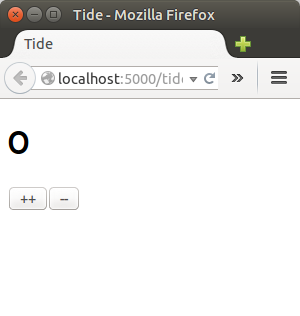
\includegraphics[width=1.0\textwidth]{images/tide-counter.png}\caption{file:$/$$/$images$/$tide-counter.png.\label{images/tide-counter.png}}\end{center}
\end{figure}

\part{ More on actions}\part{ Managing sessions}\part{ Handlers}
\begin{todo}

should it be there already? It seems too early to talk about that, but I need to introduce the concept in order to talk about the file upload handler.
\end{todo}
\part{ Creating custom Presenters}\part{ Managing file uploads}
Managing file uploads in the context of a flat-client application can be cumbersome. 
The reason is that file uploads with the HTTP protocols were not made for asynchronous 
uploads. Tide tries to solve this problem by abstracting away the implementation details 
of an AJAX-friendly file upload with the \ct{TDFileHandler} class.
\chapter{ Creating file upload entry points}\part{ Handling exceptions}\part{ A more advanced example: $<$$<$FIND SOMETHING$>$$>$}

\end{document}
